\documentclass[12pt,a4paper]{report}
\renewcommand{\baselinestretch}{2.0}

\usepackage[T1]{fontenc}
\usepackage{times,newtxmath,newtxtext}

\usepackage[utf8]{inputenc}
\usepackage{subcaption}
\usepackage{setspace}
\usepackage{multirow}
\usepackage{multicol}
\usepackage[tableposition=top]{caption}
\usepackage[table,xcdraw]{xcolor}
\usepackage{titlesec}
\usepackage{indentfirst}
\usepackage{enumitem}
\usepackage{overpic}
\usepackage{tikz}

\setlength{\parindent}{1cm}

\captionsetup[table]{labelsep=space}
\captionsetup[figure]{labelsep=space}

\usetikzlibrary{shapes.geometric, arrows}
\definecolor{blu}{RGB}{135,206,250}
\definecolor{ore}{RGB}{255,140,0}
\tikzstyle{process} = [rectangle, rounded corners, minimum width=4cm, minimum height=1cm, text centered, text width=5cm, draw=black, fill=blu]
\tikzstyle{process2} = [rectangle, rounded corners, minimum width=3cm, minimum height=1cm, text centered, text width=3cm, draw=black, fill=blu]
\tikzstyle{decision} = [diamond, minimum width=2.2cm, minimum height=0.3cm, text centered, text width=1.1cm, draw=black, fill=orange!40]
\tikzstyle{arrow} = [thick,->,>=stealth]

\usepackage{gensymb}
\usepackage{notoccite}
\usepackage{float}
\usepackage{hyperref}
\hypersetup{
    colorlinks,
    citecolor=black,
    filecolor=black,
    linkcolor=black,
    urlcolor=black,
    linkbordercolor=red
}
\usepackage{indentfirst}
\usepackage{amsmath}

\title{major}
\author{David}
\date{Juli 2022}

\renewcommand{\chaptername}{BAB }
\renewcommand{\figurename}{Gambar}
\renewcommand{\tablename}{Tabel}
\renewcommand{\contentsname}{DAFTAR ISI}
\renewcommand{\listtablename}{DAFTAR TABEL}
\renewcommand{\listfigurename}{DAFTAR GAMBAR}
\renewcommand{\bibname}{DAFTAR PUSTAKA}

\renewcommand{\thechapter}{\Roman{chapter}}
\renewcommand{\thesection}{\arabic{chapter}.\arabic{section}.}
\renewcommand{\thesubsection}{\arabic{chapter}.\arabic{section}.\arabic{subsection}.}
\renewcommand{\thesubsubsection}{\arabic{chapter}.\arabic{section}.\arabic{subsection}.\arabic{subsubsection}.}

\renewcommand{\thefigure}{\arabic{chapter}.\arabic{figure}.}
\renewcommand{\thetable}{\arabic{chapter}.\arabic{table}.}
\renewcommand{\theequation}{\arabic{chapter}.\arabic{equation}}

\usepackage{graphicx}
\usepackage[a4paper,top=40mm,bottom=30mm,left=40mm,right=30mm]{geometry}

\usepackage{tocloft}
\renewcommand{\cfttoctitlefont}{\hspace*{\fill}\Large\bfseries}
\renewcommand{\cftaftertoctitle}{\hspace*{\fill}}
\renewcommand{\cftlottitlefont}{\hspace*{\fill}\Large\bfseries}
\renewcommand{\cftafterlottitle}{\hspace*{\fill}}
\renewcommand{\cftloftitlefont}{\hspace*{\fill}\Large\bfseries}
\renewcommand{\cftafterloftitle}{\hspace*{\fill}}

\usepackage{sectsty}

\chapternumberfont{\Large} 
\chaptertitlefont{\Large}
\pagenumbering{roman}
\sectionfont{\normalsize}
\subsectionfont{\normalsize}
\titleformat{\section}{\large\bfseries}{\thesection}{1em}{}
\titlespacing\section{0pt}{12pt plus 4pt minus 2pt}{0pt plus 2pt minus 2pt}
\titlespacing\subsection{0pt}{12pt plus 4pt minus 2pt}{0pt plus 2pt minus 2pt}
\titlespacing\subsubsection{0pt}{12pt plus 4pt minus 2pt}{0pt plus 2pt minus 2pt}

\titleformat{\chapter}[display]
	{\normalfont\large\bfseries\centering}{\chaptertitlename \thechapter \centering}{-10pt}{\large}
\titlespacing*{\chapter}{0pt}{-30pt}{20pt}

\setcounter{secnumdepth}{4}
\setcounter{tocdepth}{4}

\usepackage{listings}
\usepackage{xcolor}
\definecolor{codegreen}{rgb}{0,0.6,0}
\definecolor{codegray}{rgb}{0.5,0.5,0.5}
\definecolor{codepurple}{rgb}{0.58,0,0.82}
\definecolor{backcolour}{rgb}{1,1,1}

\lstdefinestyle{mystyle}{
    backgroundcolor=\color{backcolour},   
    commentstyle=\color{codegreen},
    keywordstyle=\color{magenta},
    numberstyle=\tiny\color{codegray},
    stringstyle=\color{codepurple},
    basicstyle=\ttfamily\footnotesize,
    breakatwhitespace=false,         
    breaklines=true,                 
    captionpos=b,                    
    keepspaces=true,                 
    numbers=left,                    
    numbersep=5pt,                  
    showspaces=false,                
    showstringspaces=false,
    showtabs=false,                  
    tabsize=2
}

\lstset{style=mystyle}


\begin{document}
\newgeometry{a4paper,top=4cm,bottom=3cm,left=4cm,right=3cm}

\begin{titlepage}
\setstretch{1.5}
\thispagestyle{empty}
    \begin{center}
        \begin{large}\begin{spacing}{1}
        \textbf{JUDUL SKRIPSI}
        \end{spacing}\end{large}
                
        \vspace{4cm}
        \textbf{SKRIPSI}
        
        \vspace{1cm}
        Diajukan sebagai Salah Satu Syarat untuk Menempuh Ujian Akhir Tingkat Sarjana pada Program Studi Fisika Fakultas Matematika dan Ilmu Pengetahuan Alam Universitas Padjadjaran
                
        \vspace{1cm}
        \textbf{NAMA PENULIS\\
        140310000001}

        \vspace{2cm}
        \begin{figure}[h]
            \centering
            
\includegraphics[width=3cm]{Gambar/logo-unpad.pdf}
            \label{fig:unpadlogo}
        \end{figure}
        
        \vspace{2cm}
        \textbf{PROGRAM STUDI FISIKA\\
        FAKULTAS MATEMATIKA DAN ILMU PENGETAHUAN ALAM\\
        UNIVERSITAS PADJADJARAN\\}

        \vspace{\baselineskip}
        \textbf{\large \the\year{}}
    \end{center}
\end{titlepage}
\newpage
\chapter*{\centering LEMBAR PENGESAHAN}

\setstretch{1.5}
\thispagestyle{empty}

\addcontentsline{toc}{chapter}{LEMBAR PENGESAHAN}
\noindent \begin{tabular}{p{3cm}p{9.5cm}}
Judul \hspace{1.5cm}:&  Judul Skripsi\\
Penyusun \hspace{0.85cm}:&  Nama Penyusun\\
NPM \hspace{1.55cm}:&  140310000001 \\
Lab \hspace{1.80cm}:&  Fisika Energi / Material / Instrumentasi \\
\end{tabular}

\vspace{1cm}

\begin{center}
Jatinangor, Juli \the\year{}\\
Menyetujui, \\
\begin{multicols}{2}
	{Pembimbing Utama\\
	\vspace{2.75cm}
	\underline{Nama Dosen Pembimbing 1} \\
	NIP. 1234567 123456 1 123\\}

	{Pembimbing Pendamping\\
	\vspace{2.75cm}
	\underline{Nama Dosen Pembimbing 2} \\
	NIP. 1234567 123456 1 123\\}
\end{multicols}

\vspace{1cm}

Mengetahui, \\
Ketua Program Studi Fisika \\
Fakultas Matematika dan Ilmu Pengetahuan Alam \\
Universitas Padjadjaran \\
\vspace{2.75cm}
\underline{ Nama Kepala Program Studi } \\
NIP. 1234567 123456 1 123 \\
\end{center}

\setstretch{2}
\chapter*{\centering KATA PENGANTAR}
\addcontentsline{toc}{chapter}{KATA PENGANTAR}

Prakata berisikan ucapan terima kasih penulis skripsi kepada pihak-pihak yang telah memberikan kontribusi terhadap penulisan skripsi, baik secara institusional maupun secara akademik.

Berikut adalah contoh penulisan rincian yang berisi ucapan terima kasih: 
\begin{enumerate}
	\item Nama pembimbing 1 dan nama pembimbing 2 selaku dosen pembimbing tugas akhir,
	\item Rekan-rekan Andromeda ...
	\item Pihak lain yang tidak dapat disebutkan satu-persatu yang telah membantu baik secara langsung maupun tidak langsung, terima kasih atas segala dukungan yang diberikan kepada penulis.
\end{enumerate}

Dengan segala kerendahan hati, penulis menyadari bahwa skripsi ini masih memiliki banyak kekurangan dan jauh dari kesempurnaan. Oleh karena itu, kritik dan saran yang membangun sangat dibutuhkan oleh penulis. Semoga skripsi ini dapat bermanfaat bagi perkembangan ilmu dan teknologi serta bagi pihak-pihak yang membutuhkan.

\vspace{1cm}
\begin{flushright}
	Jatinangor, Juli \the\year{}\\
	\vspace{0.5cm}
	Penulis
\end{flushright}

\chapter*{\centering ABSTRAK}
\addcontentsline{toc}{chapter}{ABSTRAK}

\begin{spacing}{1.25}
\noindent Abstrak, merupakan sari tulisan, meliputi latar belakang penelitian secara ringkas, tujuan, metode, hasil penelitian, dan simpulan penelitian. Panjang abstrak antara 150 - 250 kata, dinyatakan dalam satu paragraf, dan dilengkapi dengan 3-5 kata kunci.\\

\noindent\textbf{Kata kunci:} Kata kunci terdiri atas 3-5 kata/frasa yang berkaitan dengan topik skripsi.
\end{spacing}
\chapter*{\centering \textit{ABSTRACT}}
\addcontentsline{toc}{chapter}{ABSTRACT}

\begin{spacing}{1.25}
\noindent\textit{Abstract merupakan versi bahasa Inggris dari Abstrak, ditulis maksimum 150-250 kata dan dilengkapi dengan keywords.\\\\
\textbf{Keywords:} Kata kunci terdiri atas 3-5 kata/frasa yang berkaitan dengan topik skripsi.}
\end{spacing}
\chapter*{\centerline{DAFTAR ISI}}
\addcontentsline{toc}{chapter}{DAFTAR ISI}

\makeatletter
\@starttoc{toc}
\makeatother

\newpage
\chapter*{\centerline{DAFTAR GAMBAR}}
\addcontentsline{toc}{chapter}{DAFTAR GAMBAR}

\makeatletter
\@starttoc{lof}
\makeatother

\newpage
\chapter*{\centerline{DAFTAR TABEL}}
\addcontentsline{toc}{chapter}{DAFTAR TABEL}

\makeatletter
\@starttoc{lot}
\makeatother

\newpage

\chapter{PENDAHULUAN}
\pagenumbering{arabic}

\section{Latar Belakang}
Latar belakang penelitian mengungkapkan keingintahuan mahasiswa tentang fenomena/gejala yang menarik untuk diteliti dengan menunjukkan signifikansi penelitian bagi pengembangan pengetahuan ilmiah. Dari pihak peneliti, pengungkapan bagian ini dapat didasarkan atas pertanyaan-pertanyaan berikut: 
\begin{enumerate}
  \item Tentang topik yang diteliti, apa-apa saja informasi yang telah diketahui, baik teoretis maupun faktual,
  \item Berdasarkan informasi yang diperoleh, adakah ditemukan adanya permasalahan baru bukan meneliti atau meniru masalah yang sudah ada,
  \item Dari permasalahan yang dapat diidentifikasi, bagian mana yang menarik untuk diteliti,
  \item Apakah mungkin secara teoretis dan teknis masalah itu diteliti,
  \item Latar Belakang harus mengarah ke identifikasi masalah.
\end{enumerate}

\section{Identifikasi Masalah}
Identifikasi masalah adalah inti fenomena yang akan diteliti sebagai akibat adanya kesenjangan teori dan realitas. Identifikasi masalah dinyatakan dalam wujud kalimat tanya yang dilengkapi dengan kata tanya; apa dan bagaimana. Misalnya:
\begin{enumerate}
  \item Apa yang hendak dibahas?
  \item Bagaimana topik tersebut ditampilkan?
\end{enumerate}

\section{Batasan Masalah}
Bagian ini menjadi salah satu bagian penting dalam Pendahuluan. Setelah paparan Latar Belakang, maka masalah yang diangkat pada pekerjaan penelitian perlu dirumuskan dengan baik. Perumusan ini sebaiknya dibahasakan tidak dalam bentuk kalimat pertanyaan, melainkan kalimat aktif, dan dapat memuat lebih dari satu rumusan. Sejalan dengan ini, setiap masalah yang diangkat selalu memiliki batas. Ada batasan, asumsi, atau kriteria yang menjadi pembatas atas masalah yang diangkat dalam penelitian TA, sehingga arah penelitian dapat fokus. Batasan ini perlu dituliskan secara tegas, dan dapat saja memuat lebih dari satu.

\section{Tujuan Penelitian}
Tujuan penelitian mengungkapkan arah dan tujuan umum apa yang akan dicapai dalam penelitian. Tujuan penelitian mengetengahkan indikator-indikator/ aspek- aspek yang hendak ditemukan dalam penelitian, terutama berkaitan dengan variabel-variabel yang akan diteliti (ditandai dengan verba yang mengindikasikan hasil; memetakan, mengklasifikasi, menunjukkan, mendeskripsikan). Tujuan Penelitian umumnya diungkapkan dalam wujud kalimat deskriptif dari identifikasi masalah.
\begin{enumerate}
  \item Mendeskripsikan topik A,
  \item Memetakan topik A.
\end{enumerate}

\chapter{TINJAUAN PUSTAKA}

\section{Penelitian Terdahulu}
Penelitian terdahulu merupakan hasil telusuran tentang kepustakaan yang mengupas topik penelitian yang relevan dengan penelitian yang akan diteliti. Hal ini merupakan bukti pendukung bahwa topik atau materi yang diteliti memang merupakan suatu permasalahan yang penting karena juga merupakan concern banyak orang, sebagaimana ditunjukkan oleh kepustakaan yang dirujuk. Penelitian terdahulu juga dapat menunjukkan posisi penelitian yang dilakukan di antara penelitian yang telah ada (\textit{state of the art}) sehingga dapat menunjukkan kebaruan (\textit{novelty}) penelitian. Penelitian terdahulu dapat bersumber dari skripsi, jurnal, prosiding, dll.

\section{Kajian Teori}
Pada bagian ini dinyatakan berbagai teori yang berkaitan dengan topik penelitian. Pada bab ini pula dimungkinkan diajukan lebih dari satu teori atau data sekunder/tersier untuk membahas permasalahan yang menjadi topik skripsi, sepanjang teori–teori dan/atau data sekunder/tersier itu berkaitan.


\chapter{METODE PENELITIAN}

\section{Objek Penelitian}
Pada bagian ini dijelaskan data/objek yang diteliti. Misalnya tahun publikasi, penulis, penerbit, summary, dll. 

\section{Metode Penelitian}
Pada bagian ini dijelaskan tahapan yang dilakukan dalam penelitian. Pada bagian ini dapat juga dijelaskan kompleksitas yang ditemukan dalam proses pengumpulan data. Hal ini penting untuk memastikan validitas data. Metode penelitian data dapat terbagi menjadi (a) metode dan teknik pengumpulan data, (b) metode dan teknik analisis data, (c) metode dan teknik penyajian hasil analisis data.
  
\chapter{HASIL DAN PEMBAHASAN}

Bagian ini menyajikan hasil penelitian dalam bentuk data. Selain dengan uraian, data penelitian dapat juga disajikan dalam bentuk ilustrasi (gambar, foto, diagram, grafik, tabel, dll.). Dalam menyajikan tabel atau grafik, hendaknya tabel dan grafik tersebut berupa self explanatory. Artinya, semua keterangan harus ada pada tabel dan grafik tersebut sehingga pembaca dapat memahaminya tanpa harus mengacu kepada teks/naskah.Yang dimaksud dengan pembahasan adalah pemaknaan terhadap data dengan mengaitkannya dengan teori yang sudah dibahas pada bab II. Temuan atau informasi yang diperoleh harus dikaitkan dengan tujuan penelitian (impikasi hasil penelitian).

\section{Gambar}

\begin{figure}[H]
  \centering
  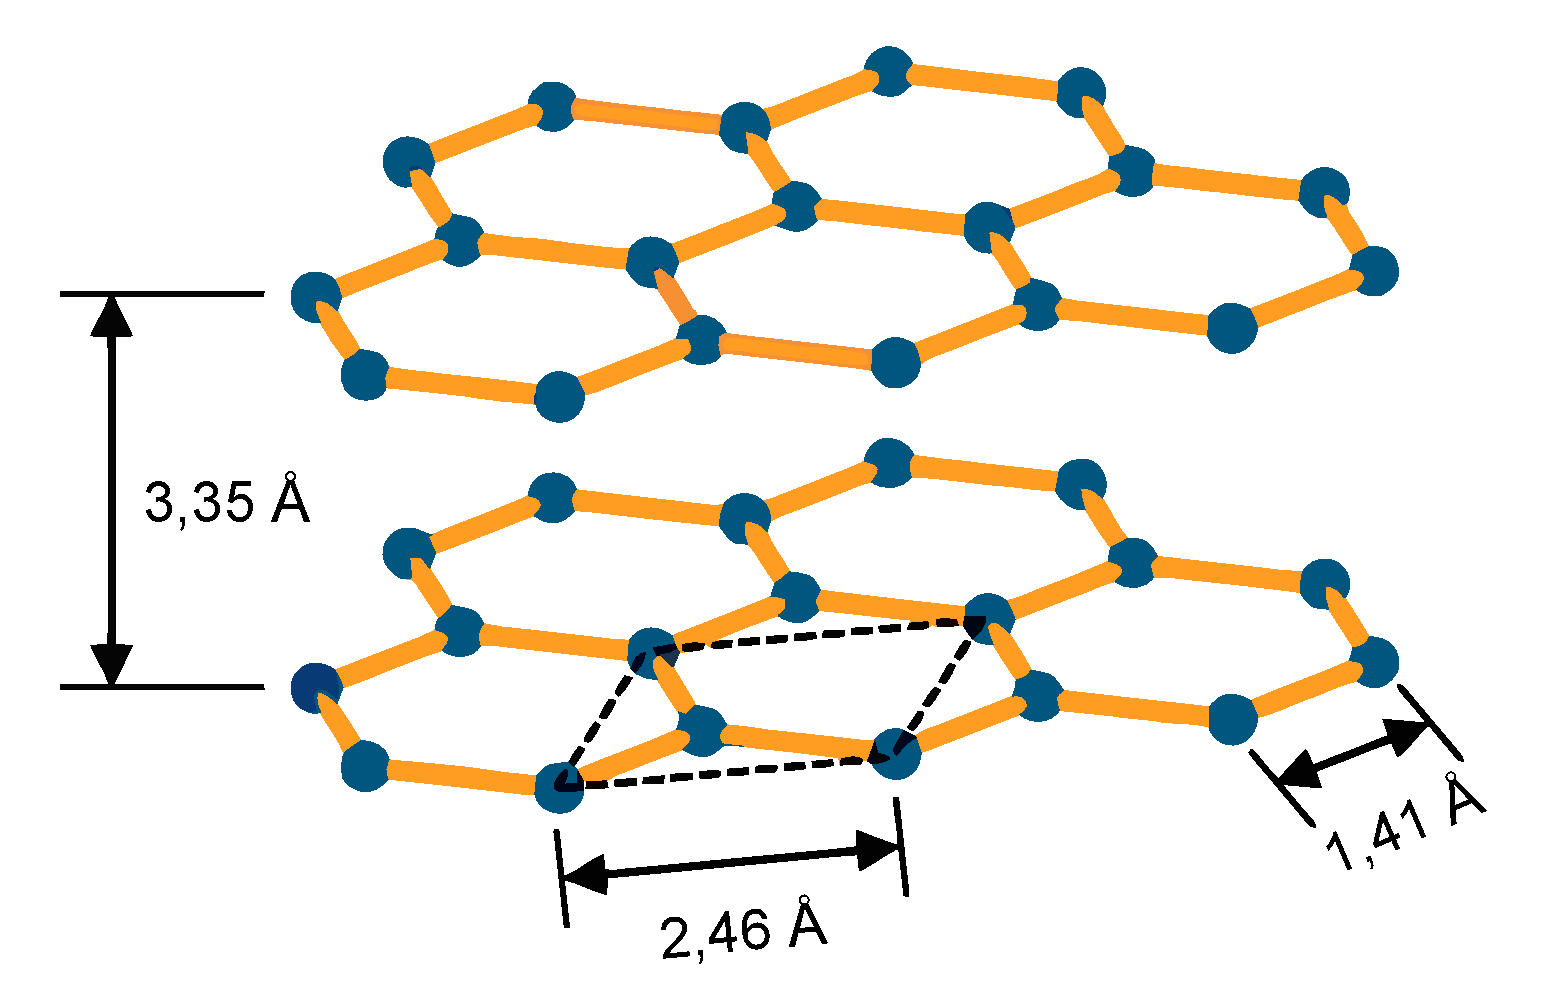
\includegraphics[width=8cm]{Gambar/blg.pdf}
  \caption{Contoh Gambar}
  \label{fig:blg}
\end{figure}

\begin{enumerate}
  \item Gambar dimuat kira-kira di tengah-tengah halaman.
  \item Judulnya ditik di bawah gambar, mengikuti lebar gambar dengan memperhitungkan keseimbangan halaman.
  \item Nomor gambar terdiri atas dua bagian, yaitu:
  \begin{enumerate}[label=(\alph*)]
    \item bagian pertama menunjukkan nomor bab tempat gambar itu dimuat;
    \item bagian kedua menunjukkan nomor urut gambar pada bab itu. Misalnya, Gambar  ~\ref{fig:blg} menunjukkan bahwa gambar itu ada pada Bab IV dan merupakan gambar urutan pertama pada bab itu.
  \end{enumerate}
  \item Kalimat pertama judul gambar ditulis dengan jarak dua ketukan sesudah nomor gambar.
  \item Awal baris kedua judul gambar berada di bawah awal judul gambar (bukan di bawah nomor gambar).
\end{enumerate}

\section{Grafik}
\begin{figure}[H]
  \begin{subfigure}{.5\textwidth}
    \centering
    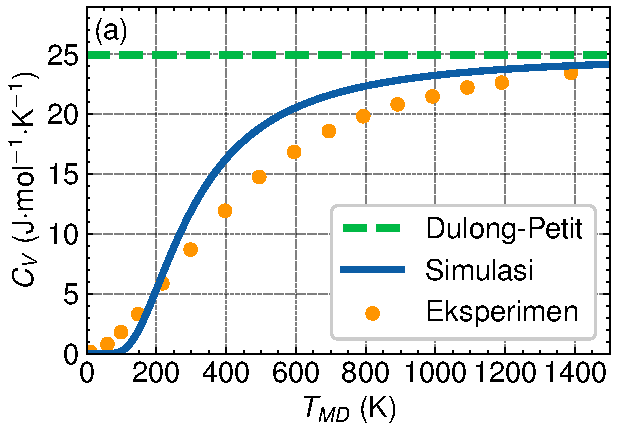
\includegraphics[width=6.7cm]{Gambar/cv.pdf}
  \end{subfigure}
  \hspace{0.7em}
  \begin{subfigure}{.5\textwidth}
    \centering
    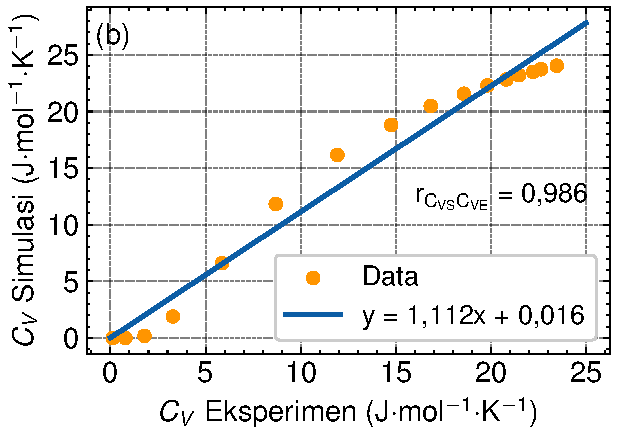
\includegraphics[width=6.7cm]{Gambar/cv_comp.pdf}
  \end{subfigure}
  \caption{Contoh Grafik}
  \label{fig:cv}
  \end{figure}

\begin{enumerate}
  \item Grafik dimuat kira-kira di tengah-tengah halaman.
  \item Judulnya ditik di atas grafik, mengikuti lebar grafik, dengan memperhitungkan keseimbangan halaman.
  \item Nomor grafik terdiri atas dua bagian, yaitu:
  \begin{enumerate}[label=(\alph*)]
    \item bagian pertama menunjukkan nomor bab grafik itu dimuat; 
    \item bagian kedua menunjukkan nomor urut grafik pada bab itu. Misalnya, Gambar  ~\ref{fig:cv} menunjukkan bahwa grafik itu ada pada Bab IV dan merupakan grafik urutan keempat pada bab itu.
  \end{enumerate}
  \item Kalimat pertama judul grafik ditulis dengan jarak dua ketukan sesudah nomor grafik.
  \item Awal baris kedua judul grafik berada di bawah awal judul grafik (bukan di bawah nomor grafik).
\end{enumerate}

\section{Tabel}
\begin{table}[ht!]
  \centering
  \caption{Contoh Tabel}
  \begin{tabular}{|l|l|l|l|l|l|}
  \hline
  \textbf{Sistem} & \textbf{m, n} & \textbf{\begin{tabular}[c]{@{}l@{}}Sudut\\ Puntir (\degree)\end{tabular}} & \textbf{\begin{tabular}[c]{@{}l@{}}Duplikasi\\ ($x \times y \times z$)\end{tabular}} & \textbf{\begin{tabular}[c]{@{}l@{}}Panjang\\ Sistem (\AA)\end{tabular}} & \textbf{\begin{tabular}[c]{@{}l@{}}Jumlah\\ Atom\end{tabular}} \\ \hline
  SLG             & -             & -                                                                  & 1 x 1 x 1                                                                & 35,98                                                                 & 434                                                            \\ \hline
  BLG          & -             & 0                                                                  & 1 x 1 x 1                                                                & 35,98                                                                 & 868                                                            \\ \hline
  tBLG            & 9, 8          & 3,89                                                               & 1 x 1 x 1                                                                & 35,98                                                                 & 868                                                            \\ \hline
  tBLG            & 8, 7          & 4,41                                                               & 1 x 1 x 1                                                                & 31,75                                                                 & 676                                                            \\ \hline
  tBLG            & 5, 3          & 16,43                                                              & 2 x 2 x 1                                                                & 34,20                                                                  & 784                                                            \\ \hline
  \end{tabular}
  \label{tab:str}
  \end{table}

\begin{enumerate}
  \item Tabel dimuat kira–kira di tengah–tengah halaman.
  \item Judulnya ditik di atas tabel, mengikuti lebar tabel, dengan memperhitungkan keseimbangan halaman.
  \item Nomor tabel terdiri atas dua bagian, yaitu:
  \begin{enumerate}[label=(\alph*)]
    \item bagian pertama menunjukkan nomor bab tabel itu dimuat;
    \item bagian kedua menunjukkan nomor urut tabel pada bab itu. Misalnya, Tabel ~\ref{tab:str} menunjukkan bahwa tabel itu berada pada Bab IV dan merupakan tabel urutan pertama pada bab itu.
  \end{enumerate}
  \item Kalimat pertama judul tabel ditulis dengan jarak dua ketukan sesudah nomor tabel.
  \item Awal baris kedua judul tabel berada di bawah awal judul tabel (bukan di bawah nomor tabel).
  \item Ukuran huruf pada isi tabel adalah 10 pt.
  \item Isi tabel ditulis dalam 1 spasi.
\end{enumerate}

\section{Persamaan}

\begin{equation}
  U_{i j}^{\mathrm{LJ}}\left(r_{i j}\right)=4 \epsilon_{i j}\left[\left(\frac{\sigma_{i j}}{r_{i j}}\right)^{12}-\left(\frac{\sigma_{i j}}{r_{i j}}\right)^{6}\right]
\end{equation}

\begin{equation}
  f_{Q}=\frac{C_v(T)}{3Nk_B}=\frac{\displaystyle\int\limits_{0}^{\infty}\frac{u^2e^u}{{(e^u-1)}^2}G(\omega)d\omega}{\displaystyle\int\limits_{0}^{\infty}G(\omega)d\omega}
\end{equation}

\section{Sitasi}
Sitasi dapat dimasukkan seperti ini \cite{moore1998cramming}. Untuk sitasi dengan beberapa sumber, dapat dituliskan juga \cite{wang2020frank,zhang2020molecular}. Atau untuk tiga sumber seperti ini \cite{mcgaughey2019phonon,jiang2015graphene,khan2015equilibrium}.
\chapter{KESIMPULAN DAN SARAN}

\section{Kesimpulan}
Simpulan merupakan kristalisasi hasil analisis dan intepretasi. Simpulan berisikan jawaban atas pertanyaan yang sudah dinyatakan pada identifikasi masalah (Bab 1). Apa yang terdapat dalam simpulan ini harus terlebih dahulu dibahas dalam bagian Pembahasan. Cara penulisan/pembahasan simpulan dirumuskan dalam bentuk pernyataan secara ketat dan padat sehingga tidak menimbulkan penafsiran lain.

\section{Saran}
Sejumlah ide yang muncul ketika melaksanakan penelitian TA dapat menjadi bahan atau topik untuk pekerjaan selanjutnya. Hal ini dapat berupa perbaikan atau ragam lain dari apa yang telah dilakukan sepanjang penelitian. Sub bab ini menjadi sumber informasi penting bagi, utamanya mahasiswa, yang akan melakukan penelitian lanjutan.

\bibliographystyle{ieeetr}
\bibliography{references}
\addcontentsline{toc}{chapter}{DAFTAR PUSTAKA}

\chapter*{\centering LAMPIRAN}
\addcontentsline{toc}{chapter}{LAMPIRAN}

\section*{Lampiran 1: Contoh Lampiran Kode}
\addcontentsline{toc}{section}{Lampiran 1: Contoh Lampiran Kode}
\lstinputlisting[language=Python]{Kode/pdospy.py}
\pagebreak

\section*{Lampiran 2: Contoh Cara Menyusun Banyak Gambar}
\addcontentsline{toc}{section}{Lampiran 2: Contoh Cara Menyusun Banyak Gambar}

\begin{figure}[h]\hspace{-2em}
    \centering
    \begin{subfigure}{.3\linewidth}
      \centering
      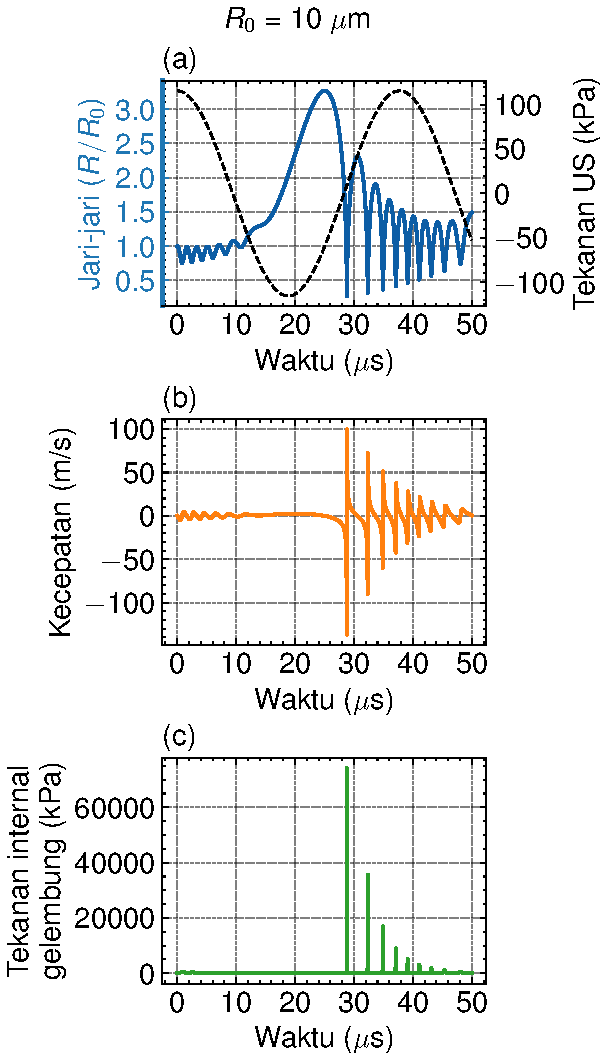
\includegraphics[width = 5.5cm]{Gambar/10.pdf}
    \end{subfigure}
    \hspace{1.5em}
    \begin{subfigure}{.3\linewidth}
      \centering
      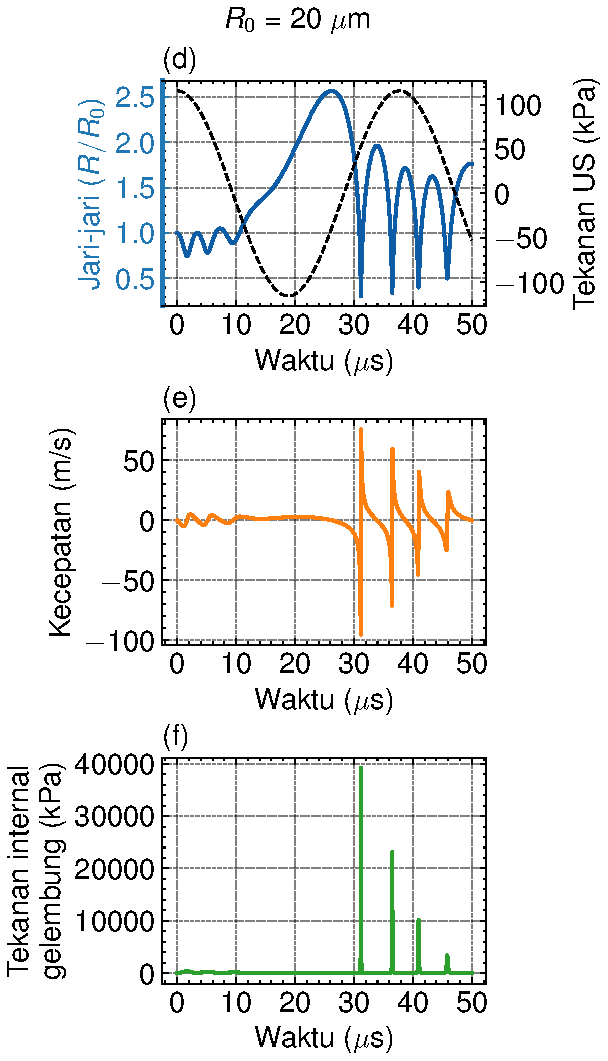
\includegraphics[width = 5.5cm]{Gambar/20.pdf}
    \end{subfigure}
    \hspace{1.5em}
    \begin{subfigure}{.3\linewidth}
      \centering
      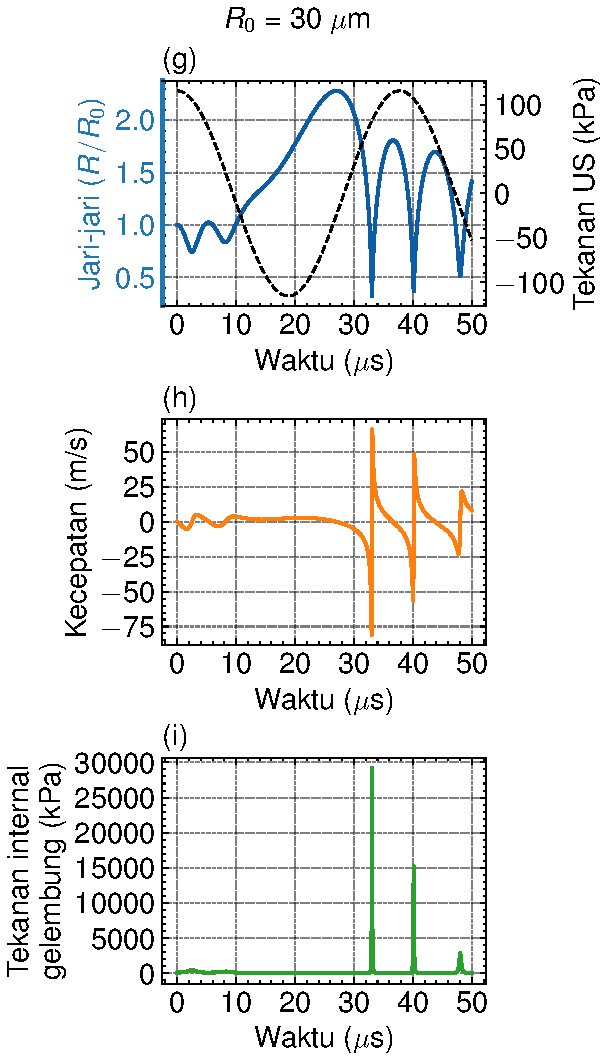
\includegraphics[width = 5.5cm]{Gambar/30.pdf}
    \end{subfigure}
  \end{figure}

\section*{Lampiran 3: Contoh Cara Menyisipkan Gambar pada Gambar}
\addcontentsline{toc}{section}{Lampiran 3: Contoh Cara Menyisipkan Gambar pada Gambar}
  \begin{figure}[H]
    \centering   
    \begin{overpic}[width=14cm]{Gambar/PDOSid.pdf}
       \put(76,14){
\includegraphics[width=1.25cm]{Gambar/gband.png}}  
    \end{overpic}
  \end{figure}
\pagebreak

\section*{Lampiran 4: Contoh Diagram}
\addcontentsline{toc}{section}{Lampiran 4: Contoh Diagram}
\begin{figure}[H]
  \centering
  \begin{tikzpicture}[node distance=2cm]
  \node (ini) [process, yshift=0.4cm] {Inisiasi};
  \node (relax) [process, below of=ini, yshift=0.4cm] {Relaksasi Struktur};
  \node (eq) [process, below of=relax, yshift=0.4cm] {Ekuilibrium};
  \node (s) [decision, below of=relax, yshift=-1.4cm] {Stabil?};
  \node (res) [process2, left of=s, xshift=-2cm] {\textit{Velocity scaling}};
  \node (prod) [process, below of=s, yshift=-0.2cm] {Produksi};
  \node (post) [process, below of=prod, yshift=0.4cm] {Hasil};
  
  \draw [arrow] (ini) -- (relax);
  \draw [arrow] (relax) -- (eq);
  \draw [arrow] (eq) -- (s);
  \draw [arrow] (s) -- node[anchor=south] {Tidak} (res);
  \draw [arrow] (res) -- +(-2,0) |- (eq);
  \draw [arrow] (s) -- node[right] {Ya} (prod);
  \draw [arrow] (prod) -- (post);
  \end{tikzpicture}
  \end{figure}
  
\end{document}
